\documentclass[xcolor=pdflatex,dvipsnames,table]{beamer}
\usepackage{epsfig,graphicx}
\usepackage{palatino}
\usepackage{fancybox}
\usepackage{relsize}
\usepackage[procnames]{listings}
\usepackage{hyperref}
\usepackage{qtree}



% fatter TT font
\renewcommand*\ttdefault{txtt}
% another TT, suggested by Alex
% \usepackage{inconsolata}
% \usepackage[T1]{fontenc} % needed as well?

\usepackage[procnames]{listings}

\newcommand{\scale}{0.7}

\newif\ifbook
% shared in slides and book

\lstdefinelanguage{chisel}{
  morekeywords={abstract,case,catch,class,def,%
    do,else,extends,false,final,finally,%
    for,if,implicit,import,match,mixin,%
    new,null,object,override,package,%
    private,protected,requires,return,sealed,%
    super,this,throw,trait,true,try,%
    type,val,var,while,with,yield},
  otherkeywords={=>,<-,<\%,<:,>:,\#,@},
  sensitive=true,
  morecomment=[l]{//},
  morecomment=[n]{/*}{*/},
  morestring=[b]",
  morestring=[b]',
  morestring=[b]"""
}

\usepackage{color}
\definecolor{dkgreen}{rgb}{0,0.6,0}
\definecolor{gray}{rgb}{0.5,0.5,0.5}
\definecolor{mauve}{rgb}{0.58,0,0.82}

% Default settings for code listings
\ifbook
\lstset{%frame=lines,
  language=chisel,
  aboveskip=3mm,
  belowskip=3mm,
  showstringspaces=false,
  columns=fixed, % basewidth=\mybasewidth,
  basicstyle={\small\ttfamily},
  numbers=none,
  numberstyle=\footnotesize,
  % identifierstyle=\color{red},
  breaklines=true,
  breakatwhitespace=true,
  procnamekeys={def, val, var, class, trait, object, extends},
  % procnamestyle=\ttfamily,
  tabsize=2,
  float
}
\else
\lstset{%frame=lines,
  language=chisel,
  aboveskip=3mm,
  belowskip=3mm,
  showstringspaces=false,
  columns=fixed, % basewidth=\mybasewidth,
  basicstyle={\small\ttfamily},
  numbers=none,
  numberstyle=\footnotesize\color{gray},
  % identifierstyle=\color{red},
  keywordstyle=\color{blue},
  commentstyle=\color{dkgreen},
  stringstyle=\color{mauve},
  breaklines=true,
  breakatwhitespace=true,
  procnamekeys={def, val, var, class, trait, object, extends},
  procnamestyle=\ttfamily\color{red},
  tabsize=2,
  float
}
\fi

\lstnewenvironment{chisel}[1][]
{\lstset{language=chisel,#1}}
{}

\newcommand{\shortlist}[1]{{\lstinputlisting[nolol]{#1}}}

\newcommand{\longlist}[3]{{\lstinputlisting[float, caption={#2}, label={#3}, frame=tb, captionpos=b]{#1}}}

\newcommand{\verylonglist}[3]{{\lstinputlisting[caption={#2}, label={#3}, frame=tb, captionpos=b]{#1}}}


\hypersetup{
  linkcolor  = black,
%  citecolor  = blue,
  urlcolor   = blue,
  colorlinks = true,
}

\newcommand{\code}[1]{{\texttt{#1}}}

\beamertemplatenavigationsymbolsempty
\setbeamertemplate{footline}[frame number]

\newcommand{\todo}[1]{{\emph{TODO: #1}}}
\newcommand{\martin}[1]{{\color{blue} Martin: #1}}
\newcommand{\abcdef}[1]{{\color{red} Author2: #1}}

% uncomment following for final submission
%\renewcommand{\todo}[1]{}
%\renewcommand{\martin}[1]{}
%\renewcommand{\author2}[1]{}


\title{Basic Digital Circuits in Chisel}
\author{Martin Schoeberl}
\date{\today}
\institute{Technical University of Denmark\\
Embedded Systems Engineering}

\begin{document}

\begin{frame}
\titlepage
\end{frame}


\begin{frame}[fragile]{Overview}
\begin{itemize}
\item Quick repeat of last lecture
\begin{itemize}
\item If something is unclear, please ask!
\end{itemize}
\item Basic digital building blocks
\item TODOs
\item go through the book
\item when and switch and so on
\item WireDefault
\item Have a ref to the Java lecture
\item The main program (compare Java with Scala)
\item Introduce vending machine (maybe next time)
\end{itemize}
\end{frame}

\begin{frame}[fragile]{The Digital Abstraction}
\begin{columns}
 
\column{0.5\textwidth}
\begin{itemize}
\item Just two values: 0 and 1, or low and hight
\item Represented as voltage
\item Digital signals tolerate noise
\item Digital Systems are \emph{simple}, just:
\begin{itemize}
\item Combinational circuits and
\item Registers
\end{itemize}
\end{itemize}
 
\column{0.5\textwidth}
\begin{figure}
  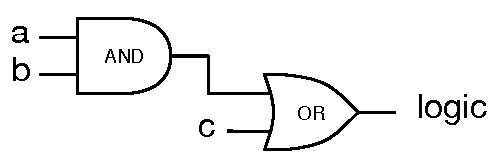
\includegraphics[scale=\scale]{../figures/logic}
\end{figure}
\begin{figure}
  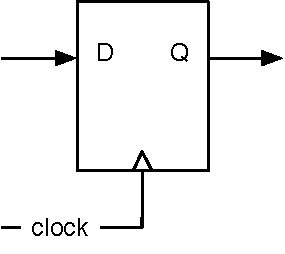
\includegraphics[scale=\scale]{../figures/register}
\end{figure}
\end{columns}

\end{frame}

\begin{frame}[fragile]{Chisel}
\begin{itemize}
\item A hardware \emph{construction} language
\begin{itemize}
\item Constructing Hardware In a Scala Embedded Language
\item If it compiles, it is synthesisable hardware 
\item Say goodby to your unintended latches
\end{itemize}
\item Chisel is not a high-level synthesis language
\item Single source for two targets
\begin{itemize}
\item Cycle accurate simulation (testing)
\item Verilog for synthesis
\end{itemize}
\item Embedded in Scala
\begin{itemize}
\item Full power of Scala available
\item But to start with, no Scala knowledge needed
\end{itemize}
\item Developed at UC Berkeley
\end{itemize}
\end{frame}

\begin{frame}[fragile]{Chisel is Part of the C Language Family}

\Tree[.C [
   [.{\bf Verilog} {\bf SystemVerilog} ]
   [.C++  \emph{SystemC}  ]
   [.Java [.Scala {\bf Chisel} ] ]
   [.C\# ] ] ]
 
\end{frame}

\begin{frame}[fragile]{Signal/Wire Types and Width}
\begin{itemize}
\item All types in hardware are a collection of bits
\item The base type in Chisel is \code{Bits}
\item \code{UInt} represents an unsigned integer
\item \code{SInt} represents a signed integer (in two's complement)
\item The number of bits is the width
\item The width written as number followed by \code{.W}
\end{itemize}
\shortlist{../code/types.txt}
\end{frame}

\begin{frame}[fragile]{Constants}
\begin{itemize}
\item Constants can represent signed or unsigned numbers
\item We use \code{.U} and \code{.S} to distinguish
\end{itemize}
\shortlist{../code/constants.txt}
\begin{itemize}
\item Constants can also be specified with a width
\end{itemize}
\shortlist{../code/const_width.txt}
\begin{itemize}
\item Use the string notation for a different base
\end{itemize}
\shortlist{../code/const_base.txt}
\end{frame}

\begin{frame}[fragile]{Combinational Circuits}
\begin{itemize}
\item Chisel uses Boolean operators, similar to C or Java
\item \code{\&} is the AND operator and \code{|} is the OR operator
\item The following code is the same as the schematics
\item \code{val logic} gives the circuit/expression the name \code{logic}
\item That name can be used in following expressions
\end{itemize}
\begin{figure}
  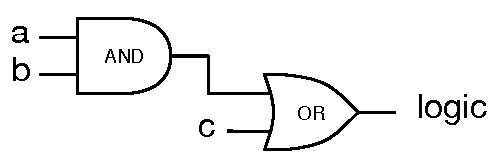
\includegraphics[scale=\scale]{../figures/logic}
\end{figure}
\shortlist{../code/logic.txt}
\end{frame}


\begin{frame}[fragile]{Arithmetic and Logic Operations}
\begin{itemize}
\item Same as in Java or C
\item But this is \emph{hardware}
\end{itemize}
\shortlist{../code/arith_ops.txt}
\shortlist{../code/bool_ops.txt}
\end{frame}

\begin{frame}[fragile]{Wires}
\begin{itemize}
\item A signal (or wire) can be first defined
\item And later assigned an expression with \code{:=}
\end{itemize}
\shortlist{../code/wire.txt}
\end{frame}

\begin{frame}[fragile]{Subfields and Concatenation}
A single bit can be extracted as follows:
\shortlist{../code/single_bit.txt}

\noindent A subfield can be extracted from end to start position:
\shortlist{../code/sub_field.txt}

\noindent Bit fields are concatenated with \code{Cat}:
\shortlist{../code/concat.txt}
\end{frame}


\begin{frame}[fragile]{A Multiplexer}
\begin{figure}
  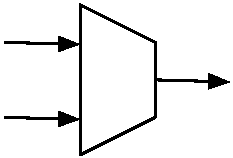
\includegraphics[scale=\scale]{../figures/mux}
\end{figure}
\begin{itemize}
\item A Multiplexer selects between alternatives
\item So common that Chisel provides a construct for it
\item Selects \code{a} when \code{sel} is \code{true.B} otherwise \code{b}
\end{itemize}
\shortlist{../code/mux.txt}
\end{frame}

\begin{frame}[fragile]{Conditional Update}
\begin{itemize}
\item With \code{when} we can express a conditional update
\item The resulting circuit is a multiplexer
\item In contrast to the \code{Mux} component, we can have several assignments in the \code{when} block
\item The rule is the the last enabled assignment counts
\begin{itemize}
\item Here the order of statements has a meaning
\end{itemize}
\end{itemize}
\shortlist{../code/comb_wire.txt}
\end{frame}

\begin{frame}[fragile]{Register}
\begin{itemize}
\item A register is a collection of flip-flops
\item Updated on the rising edge of the clock
\item May be set to a value on reset
\end{itemize}
\begin{figure}
  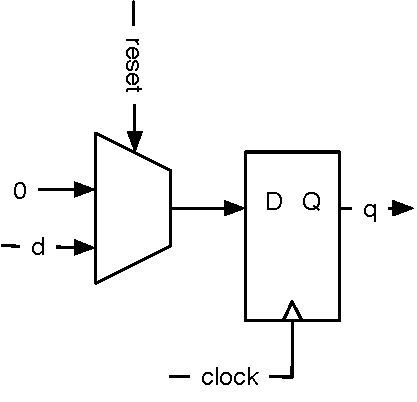
\includegraphics[scale=\scale]{../figures/register-reset-0}
\end{figure}
\end{frame}

\begin{frame}[fragile]{A Register with Reset}
Following code defines an 8-bit register, initialized with 0 at reset:
\shortlist{../code/register.txt}
\noindent An input is connected to the register with the \code{:=} update operator and
the output of the register can be used just with the name in an expression:
\shortlist{../code/reg_con.txt}
\end{frame}

\begin{frame}[fragile]{Reminder: We Construct Hardware}
\begin{itemize}
\item Chisel code looks much like Java code
\item But it is \emph{not} a program in the usual sense
\item It represents a circuit
\item We should be able to \emph{draw} that circuit
\item The ``program'' constructs the circuit
\item All statements are ``executed'' in parallel
\item Statement order has mostly no meaning
\end{itemize}
\end{frame}

\begin{frame}[fragile]{Interlude}
\begin{itemize}
\item Before we look at new material
\item Sprinkle in some general development tools
\item Get better at using your computer
\item Learn some tools
\item Don't be afraid from the command line ;-)
\item
\item
\item Engineers are power users!
\end{itemize}
\end{frame}

\begin{frame}[fragile]{What is \code{git}?}
\begin{itemize}
\item \code{git} is a distributed version-control system
\begin{itemize}
\item What does that mean?
\item \href{https://en.wikipedia.org/wiki/Git}{Wikipedia on git}
\item Draw a figure
\end{itemize}
\item To manage source code or other documents
\item Created by Linus Torvalds for Linux kernel development
\item Good tool for cooperation
\item Mostly used as the command line
\item Command line tool, but Windows clients are available
\end{itemize}
\end{frame}

\begin{frame}[fragile]{What is GitHub?}
\begin{itemize}
\item \href{https://github.com/}{GitHub} is a git server
\item GitHub is a classic startup, based in San Francisco
\item Acquired by Microsoft for \$7.5 billion
\item Many open-source projects are on GitHub (e.g., Chisel)
\begin{itemize}
\item 85 million repositories, and 28 million developers
\end{itemize}
\item Our DE2 material is hosted on GitHub
\begin{itemize}
\item Lab material (you have used it)
\item The slides
\item The Chisel book
\item see \url{https://github.com/schoeberl}
\item Everyone can contribute via GitHub ;-)
\end{itemize}
\end{itemize}
\end{frame}

\begin{frame}[fragile]{XXX}
\begin{itemize}
\item
\begin{itemize}
\item
\end{itemize}
\item
\item
\item
\item
\item
\end{itemize}
\end{frame}

\begin{frame}[fragile]{XXX}
\begin{itemize}
\item
\item
\item
\item
\item
\item
\end{itemize}
\end{frame}


\begin{frame}[fragile]{XXX}
\begin{itemize}
\item
\item
\item
\item
\item
\item
\end{itemize}
\end{frame}

\begin{frame}[fragile]{Chisel VHDL Comparison}
\begin{columns}
\column{0.5\textwidth}
\begin{chisel}
class DecodeExecute extends Bundle {
  val rs1 = UInt(32.W)
  val rs2 = UInt(32.W)
  val immVal = UInt(32.W)
  val aluOp = new AluOp()
}
\end{chisel}
\column{0.5\textwidth}
\begin{verbatim}
VHDL code here
\end{verbatim}
\end{columns}
Also show latch and and using a button as clock
\end{frame}




\begin{frame}[fragile]{Title}
\begin{itemize}
\item abc
\end{itemize}
\end{frame}

\begin{frame}[fragile]{Lab Today}
\begin{itemize}
\item Combinational circuits in Chisel
\item \href{https://github.com/schoeberl/chisel-lab/tree/master/lab2}{Lab 2 Page}
\item You need to download again, as I have updated the lab code
\item TODO: explain what it is about
\end{itemize}
\end{frame}

\end{document}

\begin{frame}[fragile]{Summary}
\begin{itemize}
\item abc
\end{itemize}
\end{frame}
